\documentclass[paper=a4, fontsize=12pt]{scrartcl}
\usepackage[T1]{fontenc}
\usepackage{fourier}
\usepackage[english]{babel}															
\usepackage[protrusion=true,expansion=true]{microtype}	
\usepackage{amsmath,amsfonts,amsthm} 
\usepackage[pdftex]{graphicx}	
\usepackage{sectsty}
\usepackage{caption}
\usepackage{subcaption}
\usepackage{geometry}
\allsectionsfont{\centering \normalfont\scshape}
\usepackage{fancyhdr}
\pagestyle{fancyplain}
\fancyhead{}											
\fancyfoot[L]{}											
\fancyfoot[C]{}											
\fancyfoot[R]{\thepage}									
\renewcommand{\headrulewidth}{0pt}			
\renewcommand{\footrulewidth}{0pt}				
\setlength{\headheight}{13.6pt}
\numberwithin{equation}{section}		
\numberwithin{figure}{section}			
\numberwithin{table}{section}			
\newcommand{\horrule}[1]{\rule{\linewidth}{#1}} 
\pagenumbering{gobble}	
\geometry{margin=1.15in}

\title{
		\vspace{-1in} 	
		\usefont{OT1}{bch}{b}{n}
		\normalfont \normalsize \textsc{Advanced Algorithms And Parallel Programmming} \\ [25pt]
		\horrule{0.5pt} \\[0.4cm]
		\huge Sudoku solver challenge \\
		\horrule{2pt} \\[0.5cm]
}
\author{
		\normalfont 								\normalsize
        Christian Rossi (10736464) - Kirolos Shroubim (10719510) - Antonio Sulfaro (10742266)\\[-3pt]		\normalsize
        \today
}
\date{}


\begin{document}
    \maketitle

    \section{Experimental setup}
    We conducted our experiments using the provided materials, which included: a set of C++ files where to write the algorithm, a bash script designed to execute the application with OpenMP that changes the number of threads, and Sudoku templates of different sizes. 
    Since we worked on a Windows system, we employed the \texttt{mingw} toolchain for compilation and used the bash CLI to manage the build and execution of the application.
    
    \section{Design choices}
    The Sudoku solver was implemented using a brute-force approach based on Depth-First Search (DFS). 
    Each empty cell in the Sudoku grid is filled by recursively attempting all valid numbers, backtracking when a conflict is encountered.
    This was achieved by creating OpenMP tasks at each recursive level. 
    However, this approach faced a major challenge: the number of tasks could grow exponentially, leading to excessive system resources usages and memory consumption.

    \noindent To address these challenges, we introduced cutoff strategies:
    \begin{itemize}
        \item \textit{Depth-based cutoff:} tasks are generated until a specific depth level is reached. 
        \item \textit{Serial algorithm cutoff:} the last levels of recursion are solved using a serial implementation. 
            This approach significantly reduces memory usage as the serial algorithm modifies the Sudoku board in place, eliminating the need to copy the board at every step.
        \item \textit{Combination of cutoffs:} a combination of the depth-based and serial cutoffs was also implemented to test their combined effectiveness, in two variations: strict (the cutoffs occurs on a higher level of depth), and very strict (even higher level).
    \end{itemize}
    These design choices allowed us to systematically explore the trade-offs between parallelism, memory usage, and computational overhead. 

    \section{Performance measurment}
    The performance of our Sudoku solver was evaluated on inputs of varying sizes: $9\times 9$, $16\times 16$, and $25\times 25$ grids. 
    All measurements were performed on a machine with the following specifications: 
    \begin{table}[!ht]
        \centering
        \begin{tabular}{|l|l|}
        \hline
        \textbf{OS}  & Microsoft Windows 11 Home                                                \\ \hline
        \textbf{CPU} & Intel Core i5-1035G1 1.00GHz, 4 Cores, 8  Logical processors \\ \hline
        \textbf{RAM} & DDR4 8.0 GB                                                               \\ \hline
        \end{tabular}
    \end{table}

    The cases taken into account are:
    \begin{enumerate}
        \item \textit{$9\times 9$ Sudoku:} this size was trivial for all configurations, with execution times consistently close to zero. 
            Due to its simplicity, it did not allow us to meaningfully observe the effects of parallelization or cutoff strategies.
        \item \textit{$16\times 16$ Sudoku:} this input size provided a better benchmark for evaluating performance.
            We observe a significant difference in the running times of algorithms with and without a serial cutoff. 
            The configuration without a cutoff shows no improvement when an additional thread is introduced, underscoring the overhead caused by excessive task creation. 
            In contrast, adopting a serial approach at lower levels of recursion drastically reduces running time. 
            Notably, the strict versions outperform the non-strict ones.
        \item \textit{$25\times 25$ Sudoku:} this input proved to be highly resource-intensive, especially with the configuration using the non-serial cutoff. 
            This implementation caused the system to crash, so we were unable to test those scenarios. 
            However, the configurations with a cutoff demonstrated significant improvement as the number of threads increased.
            Interestingly, the best performance was observed with the non-strict cutoff configuration.
    \end{enumerate}
    The performance measure of the algorithm in the given machine are as follows: 
    \begin{figure}[!ht]
        \centering
        \begin{subfigure}[b]{0.49\textwidth}
            \centering
            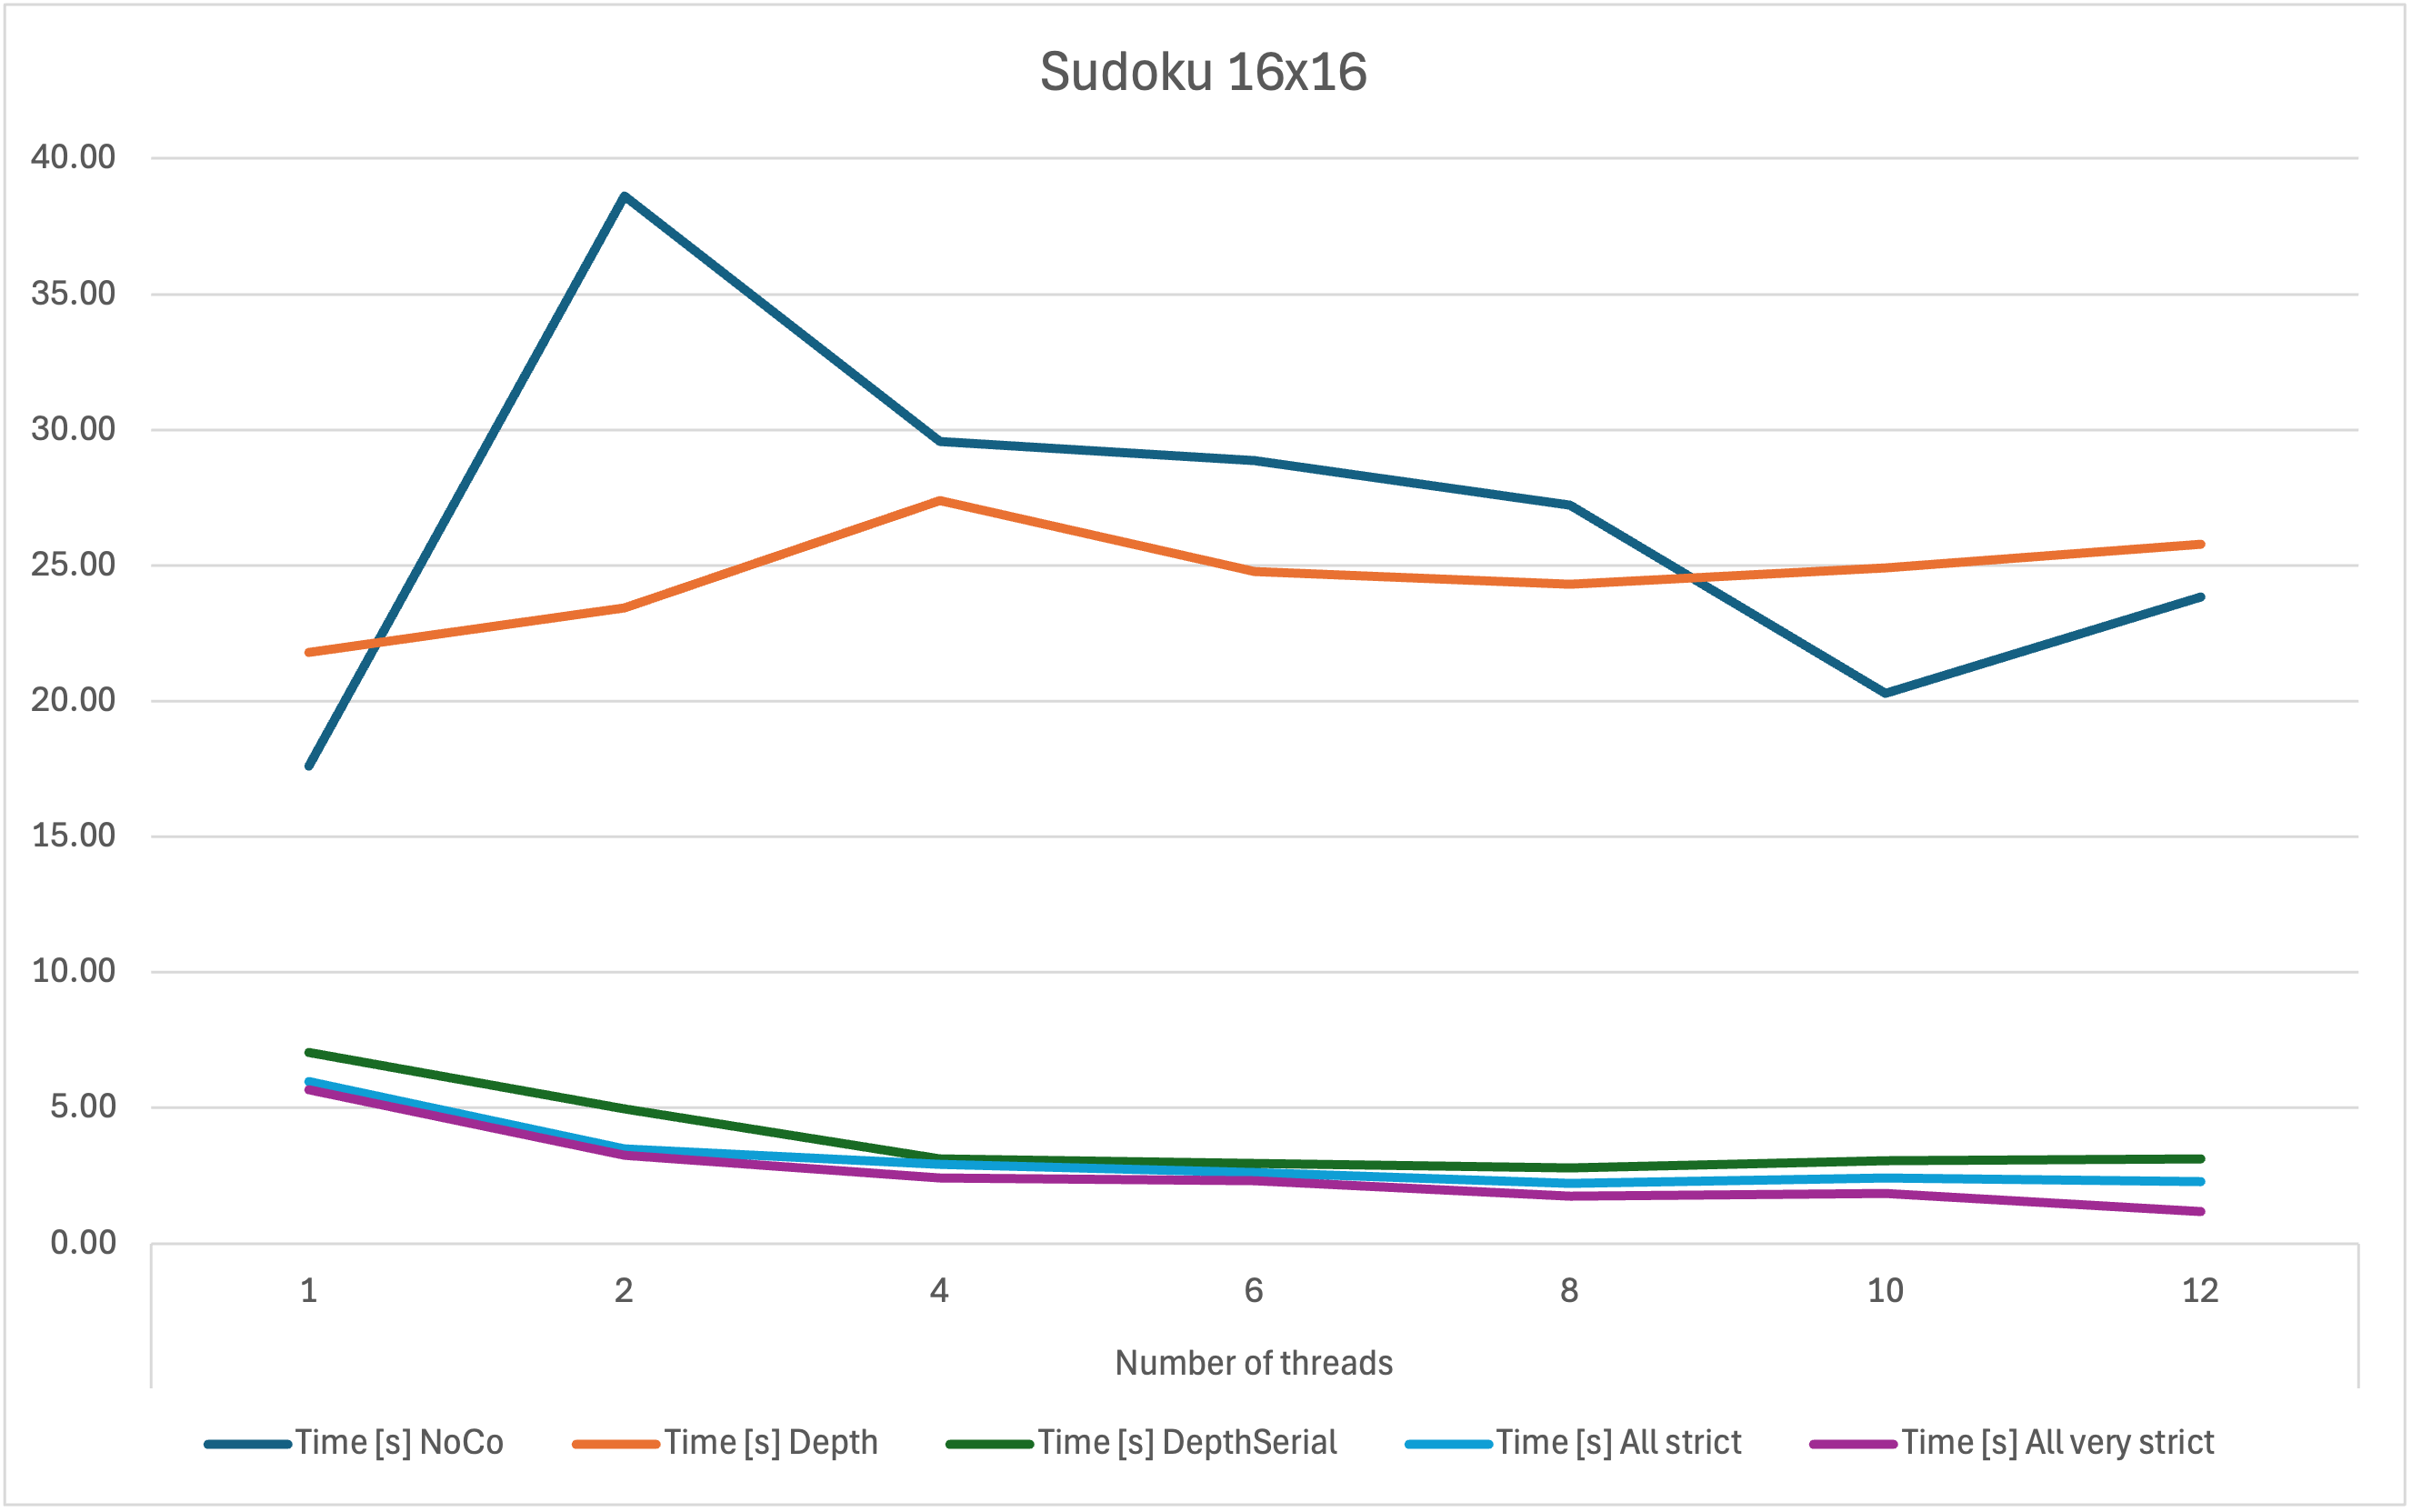
\includegraphics[width=\textwidth]{image16.png} 
        \end{subfigure}
        \hfill
        \begin{subfigure}[b]{0.49\textwidth}
            \centering
            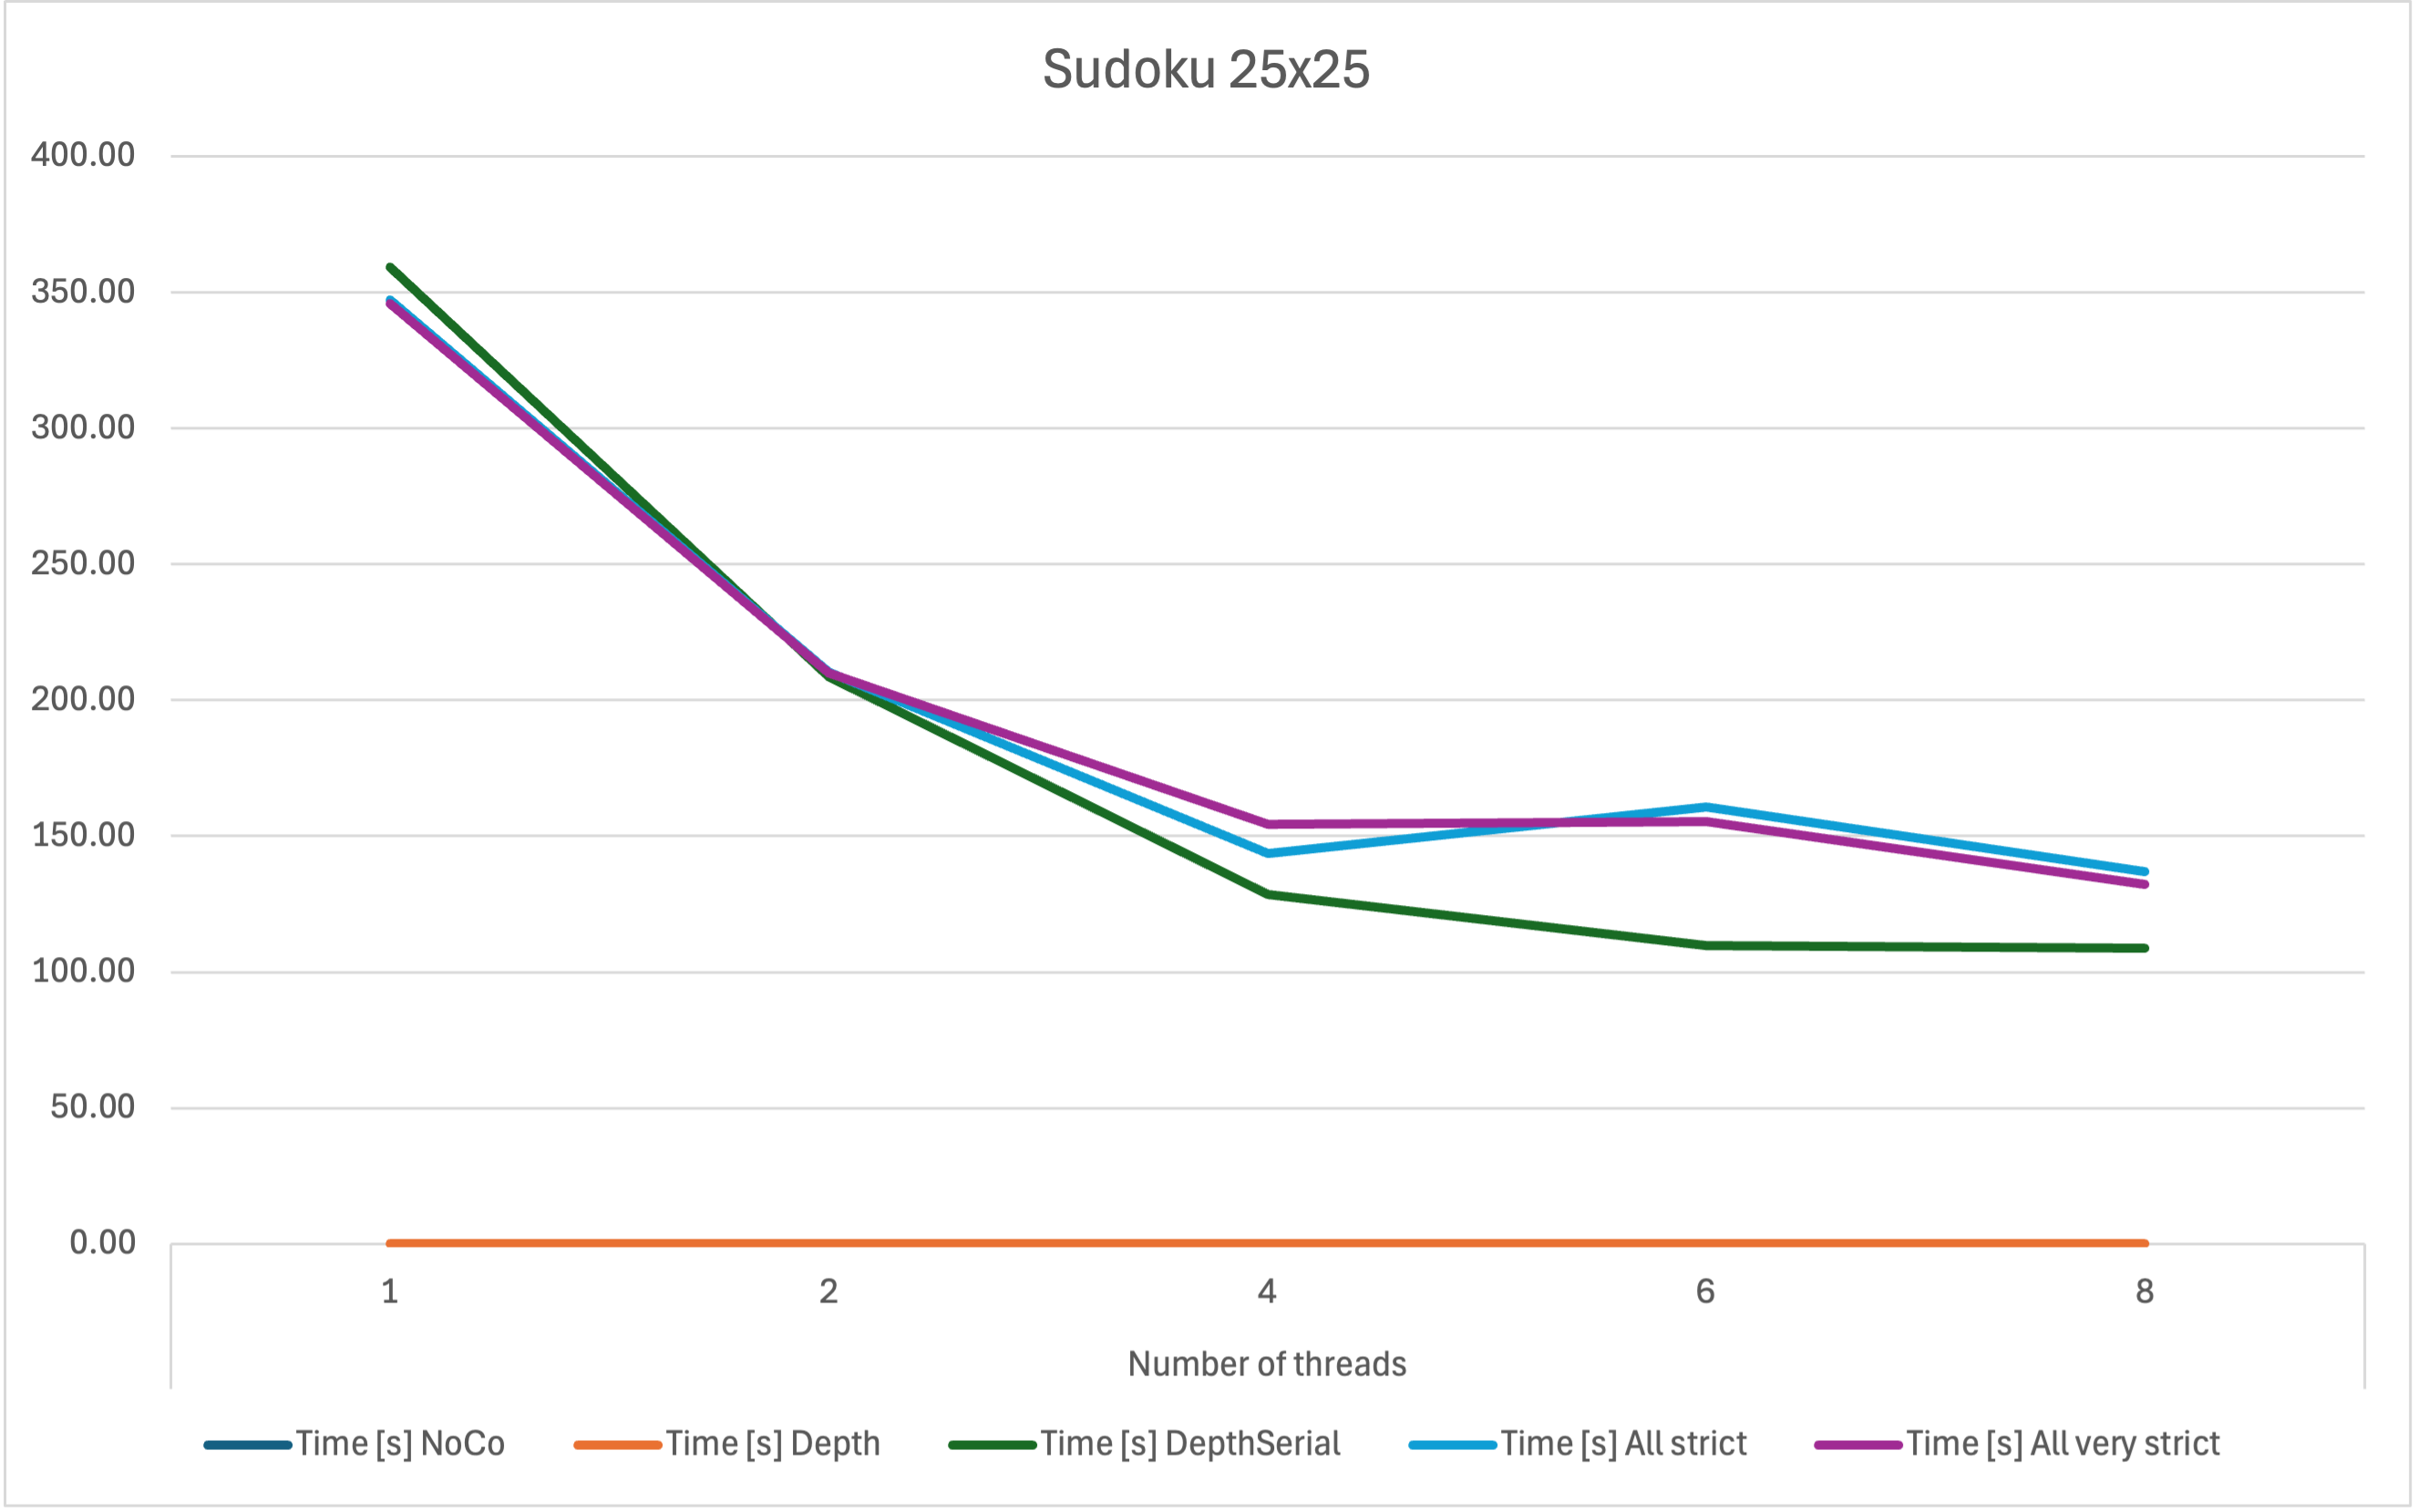
\includegraphics[width=\textwidth]{image25.png} 
        \end{subfigure}
        \caption{Performance for Intel Core i5}
    \end{figure}
    The performance of the algorithm varied significantly across different hardware setups.
    This variability demonstrates that parallel algorithms must be fine-tuned for the specific machine they are run on.
\end{document}